\documentclass[8pt]{beamer}
\usepackage[utf8]{inputenc}

\usepackage{amsmath}
\usepackage{amsfonts}
\usepackage{amssymb}
\usepackage{graphicx}
\usepackage{subfig}
\usepackage{lipsum}
\usepackage{ragged2e}
\usepackage{hyperref}
\usepackage{float}
\usepackage{url}
%\usetheme{PaloAlto}
\usepackage{amsmath,amssymb,enumerate,epsfig,bbm,calc,color,ifthen,capt-of}
\usepackage[spanish]{babel}
\usetheme{Berlin}
%\usetheme{Copenhagen}
%\usetheme{Pittsburgh}
%\usetheme{Singapore}
\usecolortheme{dolphin}
%\usecolortheme{seahorse}

\newcommand{\celda}[1]{
\begin{minipage}{2.5cm}
\vspace{5mm}
#1
\vspace{5mm}
\end{minipage}
}



\author[Jhon]{Jhon Gesell Villanueva Portella\inst{1}}
\title[Fundamentos de Programación I]{JavaScript}
\date{08 de julio de 2020} 
\subtitle{Introducción, Operadores básicos y Programación orientada a objetos}
\logo{
\includegraphics[scale=0.05]{logo_tls_web1.png}}
\institute[TLS]{
\inst{1}
Tolouse Lautrec. \\Diseño. \\Diseño y Desarrollo para Medios Digitales.\\
\vspace{2mm}

}
\AtBeginSection[]
{
\begin{frame}<beamer>{Contenido}
\tableofcontents[currentsection,currentsubsection]
\end{frame}
}


\begin{document}
\begin{frame}
\maketitle
\end{frame}
\begin{frame}{Contenido}
\tableofcontents
\end{frame}
\section{Introducción}
\begin{frame}{Introducción 01/02}
\justifying
El lienzo le permite dibujar objetos gráficos (por ejemplo, líneas, rectángulos, círculos) y animarlos, el lienzo está integrado en todos los navegadores modernos, por lo que no hay que instalar un software adicional para que los usuarios finales puedan tratar.

{\tiny Web Programming with html5, css, and javascript de John Dean (2019), pág. 570}

Canvas es un elemento HTML incorporado en HTML5 que permite la generación de gráficos dinámicamente por medio del scripting. Entre otras cosas, permite la renderización interpretada dinámica de gráficos 2D y mapas de bits, así como animaciones con estos gráficos. Wikipedia

{\tiny Wikipedia (2020)}
\end{frame}

\begin{frame}{Introducción 02/02}
\justifying
El lienzo le permite dibujar objetos gráficos (por ejemplo, líneas, rectángulos, círculos) y animarlos, el lienzo está integrado en todos los navegadores modernos, por lo que no hay que instalar un software adicional para que los usuarios finales puedan tratar.

{\tiny Web Programming with html5, css, and javascript de John Dean (2019), pág. 570}
\end{frame}

\begin{frame}{Sintáxis básica canvas 01/03}
\justifying
Para usar el lienzo, necesita (1) un elemento del lienzo y (2) llamadas al método JavaScript que dibujan objetos gráficos dentro del área de dibujo del elemento del lienzo. Aquí hay un elemento de lienzo de ejemplo, que crea un área de dibujo rectangular en blanco de 480 píxeles por 250 píxeles en una página web:

\begin{figure}[H]
\centering
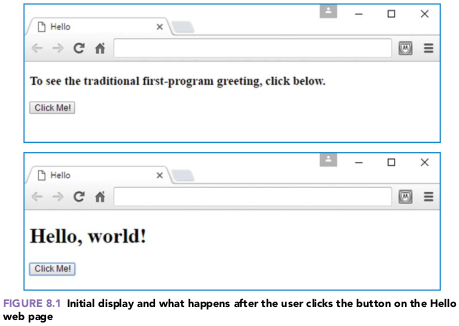
\includegraphics[scale=0.5]{Section_Files/images/Sec01/01.png}
\end{figure}


{\tiny Web Programming with html5, css, and javascript de John Dean (2019), pág. 571}
\end{frame}

\begin{frame}{Sintáxis básica canvas 02/03}
\justifying
Después de que se carga la página web, el evento onload se activa y llama a la función rectangleExamples, que dibuja formas rectangulares dentro del área de dibujo del lienzo. Examinaremos la función rectangleExamples en la siguiente sección. Como habrás adivinado, el atributo id del elemento del lienzo permite que la función acceda al objeto del lienzo. Tenga en cuenta el texto que aparece entre las etiquetas del elemento del lienzo. Ese es el contenido alternativo. Se muestra cuando el navegador del usuario no admite el elemento de lienzo. Si necesita admitir navegadores antiguos, debe incluir dicho contenido alternativo, pero dado que todos los navegadores modernos admiten lienzo,

{\tiny Web Programming with html5, css, and javascript de John Dean (2019), pág. 571}
\end{frame}

\begin{frame}{Sintáxis básica canvas 03/03}
\justifying
Hay dos tipos de comandos de dibujo de lienzo: los que dibujan imágenes bidimensionales y los que dibujan imágenes tridimensionales. Vamos a mantener las cosas simples y seguir con las imágenes bidimensionales. Para crear imágenes bidimensionales, recupera el contexto bidimensional del lienzo de esta manera:

\begin{figure}[H]
\centering
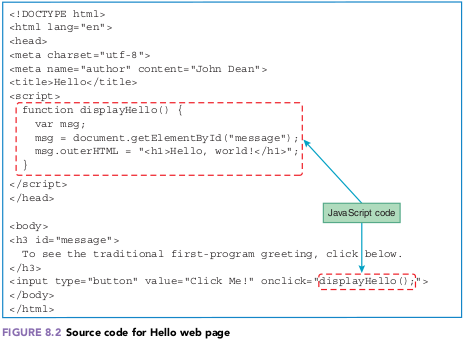
\includegraphics[scale=0.5]{Section_Files/images/Sec01/02.png}
\end{figure}

Normalmente, debe mantenerse alejado de las abreviaturas oscuras para nombres de variables, pero ctx es una abreviatura estándar para el contexto de un lienzo.

{\tiny Web Programming with html5, css, and javascript de John Dean (2019), pág. 572}
\end{frame}


\section{Operaciones Básicas}
\begin{frame}{Introducción}
\justifying
Comenzamos el capítulo con una discusión sobre el objeto de la ventana, que permite al programador recuperar información sobre la ventana del navegador: la URL de la página web actualmente activa, el tipo de navegador, etc. Luego pasamos a los cuadros de diálogo, que proporcionan un medio crudo, pero efectivo, para obligar al usuario a responder una pregunta. Introducimos la declaración if para hacer cosas diferentes, dependiendo de la respuesta del usuario a una pregunta. Luego hablamos de cadenas y números. Para obligar a los usuarios a proporcionar información que tenga sentido, describimos técnicas de validación de restricción de entrada. Finalmente, hablamos de varios operadores que pueden usarse con la declaración if para distinguir entre diferentes situaciones.


{\tiny Web Programming with html5, css, and javascript de John Dean (2019)}
\end{frame}

\begin{frame}{Objeto Ventana 01/02}
\justifying
\begin{figure}[H]
\centering
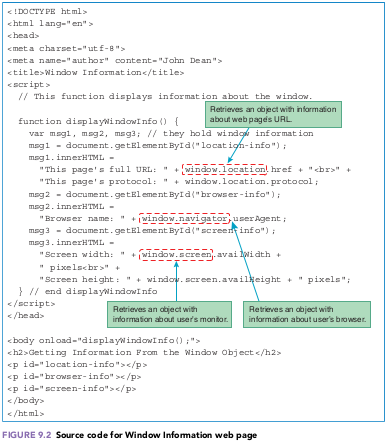
\includegraphics[scale=0.4]{Section_Files/images/Sec02/01.png}
\caption{Código fuente de una ventana.}
\end{figure}


{\tiny Web Programming with html5, css, and javascript de John Dean (2019)}
\end{frame}

\begin{frame}{Objeto Ventana 02/02}
\justifying
\begin{figure}[H]
\centering
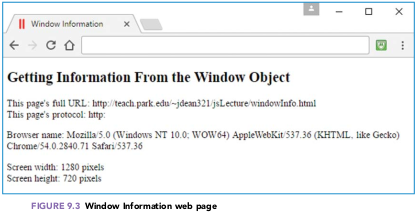
\includegraphics[scale=0.5]{Section_Files/images/Sec02/02.png}
\caption{Información de una ventana.}
\end{figure}


{\tiny Web Programming with html5, css, and javascript de John Dean (2019)}
\end{frame}

\begin{frame}{Método de alerta y confirmación}
\justifying
Diapositiva 02


{\tiny Web Programming with html5, css, and javascript de John Dean (2019)}
\end{frame}

\begin{frame}{Declaración 'if'}
\justifying
Diapositiva 03


{\tiny Web Programming with html5, css, and javascript de John Dean (2019)}
\end{frame}

\begin{frame}{Página web juego nocturno}
\justifying
Diapositiva 04


{\tiny Web Programming with html5, css, and javascript de John Dean (2019)}
\end{frame}

\begin{frame}{Método 'prompt'}
\justifying
Diapositiva 05


{\tiny Web Programming with html5, css, and javascript de John Dean (2019)}
\end{frame}

\begin{frame}{Página web juego nocturno, revisado}
\justifying
Diapositiva 06


{\tiny Web Programming with html5, css, and javascript de John Dean (2019)}
\end{frame}

\begin{frame}{Declaración 'if', 'else'}
\justifying
Diapositiva 07


{\tiny Web Programming with html5, css, and javascript de John Dean (2019)}
\end{frame}

\begin{frame}{Strings}
\justifying
Diapositiva 08


{\tiny Web Programming with html5, css, and javascript de John Dean (2019)}
\end{frame}

\begin{frame}{Página web ordenando palabras}
\justifying
Diapositiva 09


{\tiny Web Programming with html5, css, and javascript de John Dean (2019)}
\end{frame}


\begin{frame}{Más detalles de strings}
\justifying
Diapositiva 10


{\tiny Web Programming with html5, css, and javascript de John Dean (2019)}
\end{frame}

\begin{frame}{Operadores aritméticos}
\justifying
Diapositiva 11


{\tiny Web Programming with html5, css, and javascript de John Dean (2019)}
\end{frame}

\begin{frame}{Método del objeto math}
\justifying
Diapositiva 12


{\tiny Web Programming with html5, css, and javascript de John Dean (2019)}
\end{frame}

\begin{frame}{Parseando números}
\justifying
Diapositiva 13


{\tiny Web Programming with html5, css, and javascript de John Dean (2019)}
\end{frame}

\begin{frame}{Página web Water Balloons}
\justifying
Diapositiva 14


{\tiny Web Programming with html5, css, and javascript de John Dean (2019)}
\end{frame}

\begin{frame}{title}
\justifying
Diapositiva 15


{\tiny Web Programming with html5, css, and javascript de John Dean (2019)}
\end{frame}

\begin{frame}{title}
\justifying
Diapositiva 16


{\tiny Web Programming with html5, css, and javascript de John Dean (2019)}
\end{frame}

\begin{frame}{title}
\justifying
Diapositiva 17


{\tiny Web Programming with html5, css, and javascript de John Dean (2019)}
\end{frame}

\begin{frame}{title}
\justifying
Diapositiva 18


{\tiny Web Programming with html5, css, and javascript de John Dean (2019)}
\end{frame}

\begin{frame}{title}
\justifying
Diapositiva 19


{\tiny Web Programming with html5, css, and javascript de John Dean (2019)}
\end{frame}

\begin{frame}{title}
\justifying
Diapositiva 20


{\tiny Web Programming with html5, css, and javascript de John Dean (2019)}
\end{frame}

\begin{frame}{title}
\justifying
Diapositiva 21


{\tiny Web Programming with html5, css, and javascript de John Dean (2019)}
\end{frame}
%\section{Controles}
%\begin{frame}{Introducción}
\justifying
Texto

\begin{figure}[H]
\centering
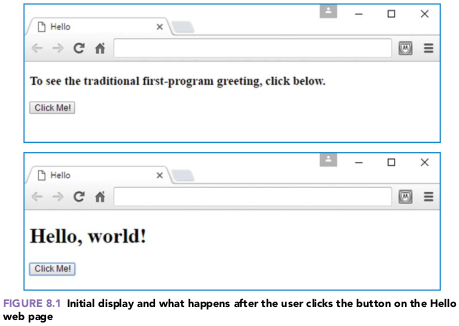
\includegraphics[scale=0.5]{Section_Files/images/Sec01/01.png}
\caption{Pantalla del 'hola mundo'.}
\end{figure}

{\tiny Libro}
\end{frame}

\begin{frame}{Ciclo While}
\justifying
Texto

{\tiny Libro}
\end{frame}

\begin{frame}{Ficheros externos de JavaScript}
\justifying
Texto

{\tiny Libro}
\end{frame}

\begin{frame}{Página web de Interés compuesto}
\justifying
Texto

{\tiny Libro}
\end{frame}

\begin{frame}{Ciclo Do}
\justifying
Texto

{\tiny Libro}
\end{frame}

\begin{frame}{Radio buttons}
\justifying
Texto

{\tiny Libro}
\end{frame}

\begin{frame}{Checkboxes}
\justifying
Texto

{\tiny Libro}
\end{frame}

\begin{frame}{Página web de habilidades de trabajo}
\justifying
Texto

{\tiny Libro}
\end{frame}

\begin{frame}{Ciclo for}
\justifying
Texto

{\tiny Libro}
\end{frame}

\begin{frame}{Conjunto de campos y elementos de leyenda}
\justifying
Texto

{\tiny Libro}
\end{frame}

\begin{frame}{Title 11}
\justifying
Texto

{\tiny Libro}
\end{frame}

\begin{frame}{Title 12}
\justifying
Texto

{\tiny Libro}
\end{frame}

\begin{frame}{Title 13}
\justifying
Texto

{\tiny Libro}
\end{frame}

\begin{frame}{Title 14}
\justifying
Texto

{\tiny Libro}
\end{frame}

\begin{frame}{Title 15}
\justifying
Texto

{\tiny Libro}
\end{frame}

\begin{frame}{Title 16}
\justifying
Texto

{\tiny Libro}
\end{frame}

\begin{frame}{Title 17}
\justifying
Texto

{\tiny Libro}
\end{frame}

\begin{frame}{Title 18}
\justifying
Texto

{\tiny Libro}
\end{frame}
\section{POO}
\begin{frame}{Introducción}
\justifying
Se definirá estructuras para nuevos tipos de objetos y usará esas estructuras para crear los objetos. Las estructuras que defina y los objetos que cree le ayudarán a organizar los datos dentro del código JavaScript de una página web. El uso de objetos para organizar datos se conoce como programación orientada a objetos (OOP). Deberá usar OOP cuando haya una cantidad significativa de datos que deba organizarse. En este capítulo, las páginas web usan más datos que en capítulos anteriores, y OOP ayudará a que el código sea más fácil de entender.

{\tiny Web Programming with html5, css, and javascript de John Dean (2019)}
\end{frame}

\begin{frame}{Generalidades de la POO}
\justifying
Como puede imaginar, si tiene una gran tarea de programación, existe un gran potencial para crear un nido de códigos intrincados. 1 En la década de 1970, los diseñadores del lenguaje de programación SmallTalk abordaron este problema de código complicado al acuñar el término programación orientada a objetos y
convirtiéndolo en una parte central de su nuevo lenguaje de programación.
El objetivo del paradigma OOP es que los programas modelen cómo las personas normales piensan sobre un problema y su solución. Al pensar en un problema, las personas tienden a centrarse en las cosas que lo componen. Con OOP, esas cosas se llaman objetos. Por lo general, son entidades físicas, pero también pueden ser entidades conceptuales. Como programador de OOP, una vez que ha identificado las cosas que desea modelar, identifica sus propiedades y comportamientos básicos. Se agrupan las propiedades y los comportamientos de cada cosa en una estructura coherente llamada objeto. Al escribir un programa OOP, usted define objetos, los crea y hace que interactúen entre sí.
Por ejemplo, si está escribiendo un programa para asignar cursos a las aulas, probablemente necesitará objetos del curso y objetos de la sala. Los objetos del curso contendrían propiedades del nombre del curso y del número de estudiantes, y los objetos de la sala contendrían propiedades de ubicación y capacidad. Los comportamientos de un objeto se refieren a las actividades asociadas con el objeto. Para un objeto del curso, probablemente necesitará un comportamiento que ajuste la propiedad del número de estudiantes del curso, ya que los estudiantes agregan y abandonan los cursos antes del primer día de clase. Con JavaScript, implementa los comportamientos de un objeto como métodos.


{\tiny Web Programming with html5, css, and javascript de John Dean (2019)}
\end{frame}

\begin{frame}{Generalidades de la POO}
\justifying
Una de las características fundamentales de OOP es la encapsulación. En general, la encapsulación es cuando algo está envuelto dentro de una cubierta protectora. Cuando se aplica a objetos, la encapsulación significa que los datos de un objeto están protegidos al estar ocultos dentro del objeto. Con datos ocultos, el resto del programa no puede acceder a los datos de un objeto directamente; el resto del programa se basa en los métodos del objeto para acceder a los datos. Acceder a los datos de un objeto se refiere a leer los datos o modificarlos. Suponiendo que los métodos de un objeto están bien escritos, los métodos aseguran que se acceda a los datos de manera adecuada. Al limitar el acceso al acceso "apropiado", eso hace que sea más difícil desordenar los datos de un programa, y eso genera menos errores. ¡Hurra! Ver FIGURA 11.1. Muestra cómo los métodos de un objeto forman la interfaz entre los datos del objeto
y el mundo exterior.

\begin{figure}
\centering
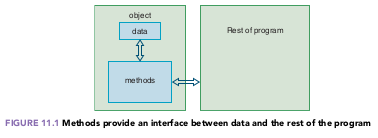
\includegraphics[scale=0.3]{Section_Files/images/Sec04/01.png}
\caption{tex1.}
\end{figure}

{\tiny Web Programming with html5, css, and javascript de John Dean (2019)}
\end{frame}

\begin{frame}{Classes, Constructores, Propiedades, nuevos
Operadores y Metodos}
\justifying

\begin{figure}
\centering
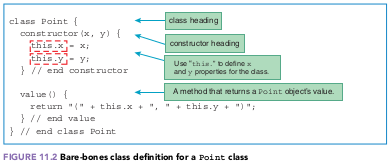
\includegraphics[scale=0.3]{Section_Files/images/Sec04/02.png}
\caption{tex1.}
\end{figure}

{\tiny Web Programming with html5, css, and javascript de John Dean (2019)}
\end{frame}
%\section{Canvas}
%\begin{frame}{Soluciones aproximadas de la ecuación de Navier Stokes}
\justifying

\begin{figure}[H]
\centering
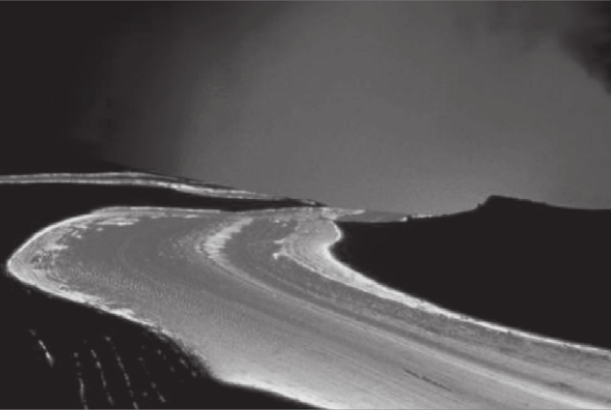
\includegraphics[scale=0.2]{Section_Files/S3-imagenes-Jhon/0001.png}
\caption{El flujo de lava de un volcán es un ejemplo de flujo trepador: la viscosidad de la roca fundida es tan grande que el número de Reynolds es pequeño aún cuando las escalas de longitud sean grandes.}
\end{figure}

{\tiny Mecánica de fluidos por Yunus A. Cengel, John M. Cimbala, pág. 491}
\end{frame}

%***************************
\begin{frame}{01. Introducción | 01/03}
\justifying
La mayoría de los problemas prácticos de la mecánica de fluidos no puede resolverse de manera analítica y demanda ya sea 1) mayores aproximaciones o 2) ayuda de computadora. Consideraremos a los flujos en estudio como incompresibles del tipo de fluido newtonianos.


Una solución aproximada se define como aquella donde la ecuación de Navier-Stokes se simplifica en alguna región del flujo antes de inclusive comenzar la solución. En otras palabras se comienzan a eliminar terminos dependiendo de la clase de problema, el cual puede diferir una región del flujo a otra.

Los fluidos estáticos pueden considerarse como una solución aproximada de Navier-Stokes. La aproximación es que los términos inercial y viscoso en la ecuación de Navier-Stokes son despreciablemente pequeños en comparación con los términos de presión y gravedad.
{\tiny Mecánica de fluidos por Yunus A. Cengel, John M. Cimbala, pág. 492}
\end{frame}

\begin{frame}{01. Introducción | 02/03}
\justifying
\begin{figure}[H]
\centering
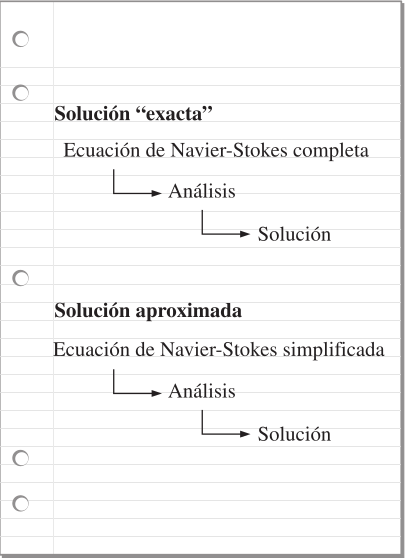
\includegraphics[scale=0.2]{Section_Files/S3-imagenes-Jhon/0002.png}
\caption{Las soluciones "exactas" comienzan con la ecuación de Navier-Stokes completa, mientras que las soluiciones aproximadas comienzan con una forma simplificada de la ecuación de Navier-Stokes justo desde el principio.}
\end{figure}

{\tiny Mecánica de fluidos por Yunus A. Cengel, John M. Cimbala, pág. 492}
\end{frame}

\begin{frame}{01. Introducción | 03/03}
\justifying
\begin{figure}[H]
\centering
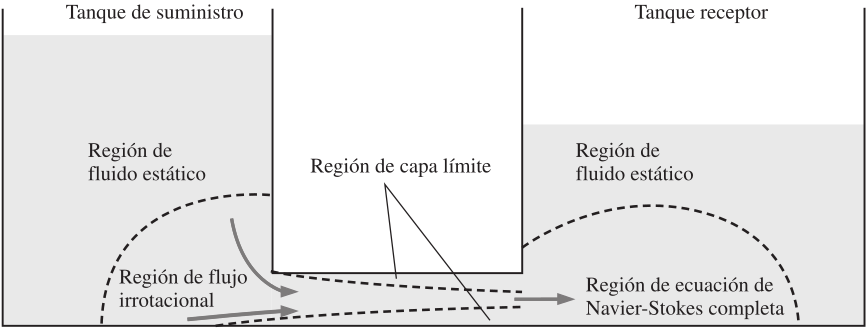
\includegraphics[scale=0.2]{Section_Files/S3-imagenes-Jhon/0003.png}
\caption{Una aproximación partícular de la ecuación de Navier-Stokes es adecuada sólo en ciertas regiones del campo de flujo; otras aproximaciones pueden no ser adecuadas en otras regiones del campo de flujo.}
\end{figure}

{\tiny Mecánica de fluidos por Yunus A. Cengel, John M. Cimbala, pág. 493}
\end{frame}


%***************************

\begin{frame}{02. Ecuaciones adimensionalizadas de movimiento | 01/04}
\justifying
Se desea eliminar las dimensiones de las ecuaciones de movimiento, de modo que puedan compararse de manera adecuada las órdenes de magnitud de los diversos términos de las ecuaciones, para ello comenzamos con la ecuación de continuidad de flujo incompresible:
\begin{figure}[H]
\centering
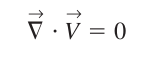
\includegraphics[scale=0.2]{Section_Files/S3-imagenes-Jhon/0004.png}
\end{figure}
y la forma vectorial de la ecuación de Navier-Stokes, valida para flujo incompresible de un fluido newtoniano con propiedades constantes:
\begin{figure}[H]
\centering
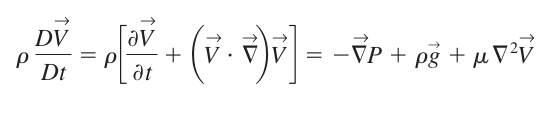
\includegraphics[scale=0.2]{Section_Files/S3-imagenes-Jhon/0005.png}
\end{figure}
{\tiny Mecánica de fluidos por Yunus A. Cengel, John M. Cimbala, pág. 493}
\end{frame}

\begin{frame}{02. Ecuaciones adimensionalizadas de movimiento | 02/04}
\justifying
Mostramos algunos parámetros de escalamiento o repetitivas característicos que se usan para eliminar las dimensiones de las ecuaciones de movimiento.
\begin{figure}[H]
\centering
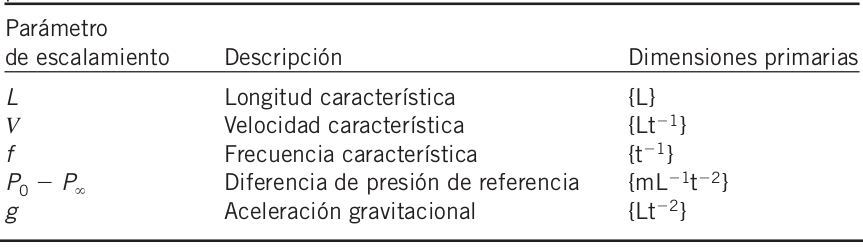
\includegraphics[scale=0.3]{Section_Files/S3-imagenes-Jhon/0006.png}
\end{figure}
{\tiny Mecánica de fluidos por Yunus A. Cengel, John M. Cimbala, pág. 494}
\end{frame}

\begin{frame}{02. Ecuaciones adimensionalizadas de movimiento | 03/04}
\justifying
Luego se definen algunas variables adimensionales y un operador adimensional con base en los parámetros de escalamiento de la tabla mostrada en el slider anterior.
\begin{figure}[H]
\centering
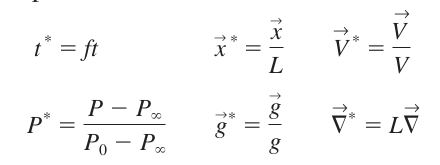
\includegraphics[scale=0.3]{Section_Files/S3-imagenes-Jhon/0007.png}
\end{figure}
{\tiny Mecánica de fluidos por Yunus A. Cengel, John M. Cimbala, pág. 494}
\end{frame}

\begin{frame}{02. Ecuaciones adimensionalizadas de movimiento | 04/04}
\justifying
Luego de haber multiplicado los terminos de la ecuación de Navier-Stokes por sus respectivos factores se obtiene.
\begin{figure}[H]
\centering
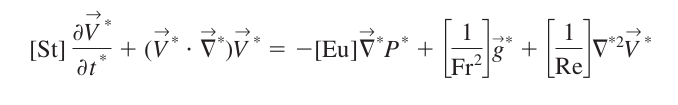
\includegraphics[scale=0.3]{Section_Files/S3-imagenes-Jhon/0015.png}
\end{figure}
{\tiny Mecánica de fluidos por Yunus A. Cengel, John M. Cimbala, pág. 495}
\end{frame}


%***************************

\begin{frame}{03. Aproximación de flujo de Stokes | 01/04}
\justifying
\begin{figure}[H]
\centering

\includegraphics[scale=0.35]{Section_Files/S3-imagenes-Jhon/0022.png}
\caption{El lento flujo de un líquido muy viscoso, en este caso la miel, se clasifica como flujo de Stokes.}
\end{figure}
%\\
{\tiny Mecánica de fluidos por Yunus A. Cengel, John M. Cimbala, pág. 496}
\end{frame}

\begin{frame}{03. Aproximación de flujo de Stokes - Ejemplo |  02/04}
\justifying
Fuerza de arrastre sobre un objeto en flujo de Stokes:
\begin{figure}[H]
\centering
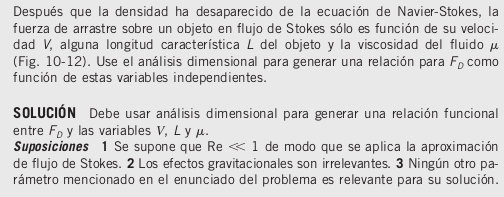
\includegraphics[scale=0.55]{Section_Files/S3-imagenes-Jhon/0027-01.png}
\end{figure}
{\tiny Mecánica de fluidos por Yunus A. Cengel, John M. Cimbala, pág. 498}
\end{frame}

\begin{frame}{03. Aproximación de flujo de Stokes - Ejemplo | 03/04}
\justifying
\begin{figure}[H]
\centering
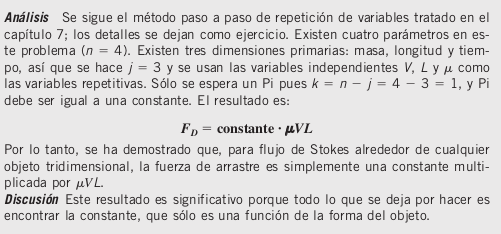
\includegraphics[scale=0.55]{Section_Files/S3-imagenes-Jhon/0027-02.png}
\end{figure}
{\tiny Mecánica de fluidos por Yunus A. Cengel, John M. Cimbala, pág. 498}
\end{frame}

\begin{frame}{03. Aproximación de flujo de Stokes - Ejemplo |  04/04}
\justifying
Fuerza de arrastre sobre un objeto en flujo de Stokes:
\begin{figure}[H]
\centering
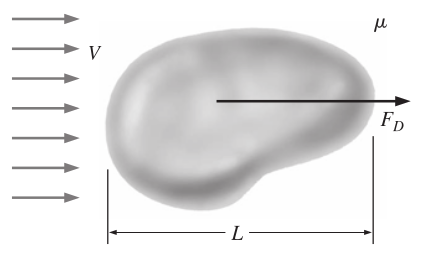
\includegraphics[scale=0.35]{Section_Files/S3-imagenes-Jhon/0031.png}
\caption{Para flujo de Stokes sobre un objeto tridimensional la fuerza de arrastre sobre el objeto no depende de la densidad, sino sólo de la velocidad $ V $, alguna longitud característica del objeto $ L $ y la viscosidad del fluido $ \mu $.}
\end{figure}
{\tiny Mecánica de fluidos por Yunus A. Cengel, John M. Cimbala, pág. 499}
\end{frame}
%***************************

\begin{frame}{Fuerza de arrastre sobre una esfera en flujo de Stokes 01/}
\justifying
\begin{figure}[H]
\centering
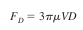
\includegraphics[scale=0.55]{Section_Files/S3-imagenes-Jhon/0031-01.png}
\caption{Fuerza de arrastre sobre una esfera en flujo de Stokes.}
\end{figure}
\begin{figure}[H]
\centering
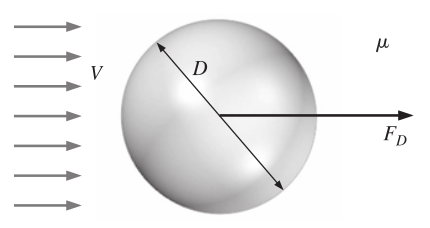
\includegraphics[scale=0.25]{Section_Files/S3-imagenes-Jhon/0032.png}
\caption{La fuerza de arrastre sobre una esfera de diámetro $ D $ en flujo de Stokes es igual a $3 \pi \mu V D$ .}
\end{figure}
{\tiny Mecánica de fluidos por Yunus A. Cengel, John M. Cimbala, pág. 499}
\end{frame}

\begin{frame}{Fuerza de arrastre sobre una esfera en flujo de Stokes - Ejemplo | 02/}
\justifying
\begin{figure}[H]
\centering
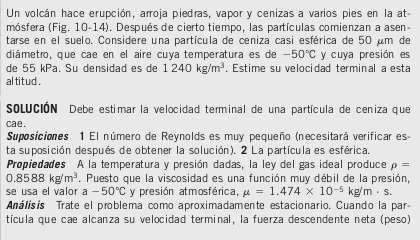
\includegraphics[scale=0.55]{Section_Files/S3-imagenes-Jhon/0032-01.png}
\end{figure}
{\tiny Mecánica de fluidos por Yunus A. Cengel, John M. Cimbala, pág. 499}
\end{frame}

\begin{frame}{Fuerza de arrastre sobre una esfera en flujo de Stokes - Ejemplo | 03/}
\justifying
\begin{figure}[H]
\centering
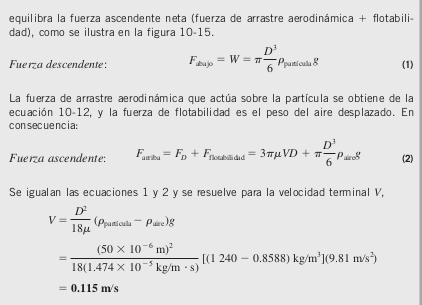
\includegraphics[scale=0.55]{Section_Files/S3-imagenes-Jhon/0032-02.png}
\end{figure}
{\tiny Mecánica de fluidos por Yunus A. Cengel, John M. Cimbala, pág. 500}
\end{frame}

\begin{frame}{Fuerza de arrastre sobre una esfera en flujo de Stokes - Ejemplo | 04}
%\justifying
\begin{figure}[H]
\centering
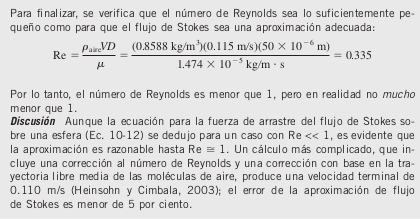
\includegraphics[scale=0.55]{Section_Files/S3-imagenes-Jhon/0032-03.png}
%\caption{La fuerza de arrastre sobre una esfera de diámetro $ D $ en flujo de Stokes es igual a $3 \pi \mu V D$ .}
\end{figure}
{\tiny Mecánica de fluidos por Yunus A. Cengel, John M. Cimbala, pág. 499}
\end{frame}

\begin{frame}{Fuerza de arrastre sobre una esfera en flujo de Stokes - Ejemplo | 05}
%\justifying
\begin{figure}[H]
\centering
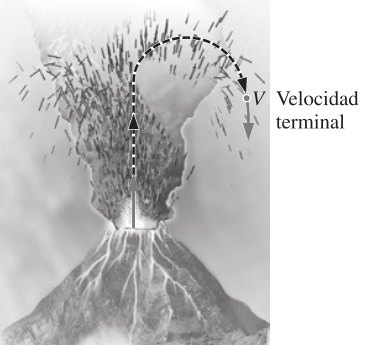
\includegraphics[scale=0.35]{Section_Files/S3-imagenes-Jhon/0033.png}
\caption{(10-14)Las partículas de ceniza que arroja una erupción volcánica se asientan lentamente en el suelo; la aproximación de flujo de Stokes es razonable para ese tipo de campo de flujo.}
\end{figure}
{\tiny Mecánica de fluidos por Yunus A. Cengel, John M. Cimbala, pág. 500}
\end{frame}

\begin{frame}{Fuerza de arrastre sobre una esfera en flujo de Stokes - Ejemplo | 06}
\justifying
\begin{figure}[H]
%\centering
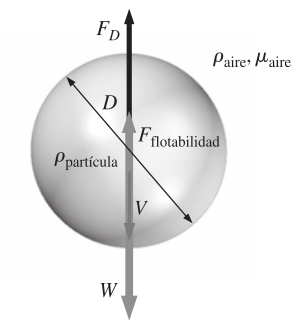
\includegraphics[scale=0.35]{Section_Files/S3-imagenes-Jhon/0034.png}
\caption{Una partícula que cae a una velocidad terminal estacionaria no tiene aceleración; en consecuencia, su peso se equilibra mediante la fuerza de arrastre aerodinámica y la de flotabilidad que actúa sobre la partícula.}
\end{figure}
{\tiny Mecánica de fluidos por Yunus A. Cengel, John M. Cimbala, pág. 500}
\end{frame}
%***************************

%\begin{frame}{04. Aproximación para regiones invíscidas de flujo}
%\justifying
%\begin{figure}[H]
%\centering
%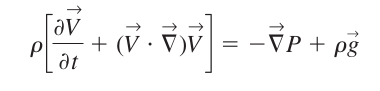
\includegraphics[scale=0.35]{Section_Files/S3-imagenes-Jhon/0035.png}
%\caption{Ecuación de Euler.}
%\end{figure}
%{\tiny Mecánica de fluidos por Yunus A. Cengel, John M. Cimbala, pág. 501}
%\end{frame}

%***************************

%\begin{frame}{Derivación de la ecuación de Bernoulli en regiones inviscidas de flujo}
%\justifying
%\begin{figure}[H]
%\centering
%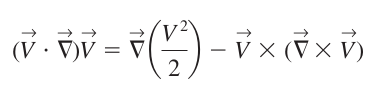
\includegraphics[scale=0.35]{Section_Files/S3-imagenes-Jhon/0037.png}
%\caption{Ecuación de Euler.}
%\end{figure}
%{\tiny Mecánica de fluidos por Yunus A. Cengel, John M. Cimbala, pág. 502}
%\end{frame}

%***************************

%\begin{frame}{05. La aproximación de flujo irrotacional}
%\justifying
%\begin{figure}[H]
%\centering
%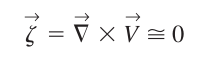
\includegraphics[scale=0.35]{Section_Files/S3-imagenes-Jhon/0048.png}
%\caption{Aproximación irrotacional.}
%\end{figure}
%{\tiny Mecánica de fluidos por Yunus A. Cengel, John M. Cimbala, pág. 505}
%\end{frame}

%***************************

%\begin{frame}{Ecuación de continuidad}
%\justifying
%\begin{figure}[H]
%\centering
%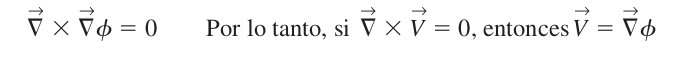
\includegraphics[scale=0.35]{Section_Files/S3-imagenes-Jhon/0049.png}
%\caption{Identidad vectorial.}
%\end{figure}
%{\tiny Mecánica de fluidos por Yunus A. Cengel, John M. Cimbala, pág. 505}
%\end{frame}

%***************************

%\begin{frame}{Ecuación de cantidad de movimiento}
%\justifying
%\begin{figure}[H]
%\centering
%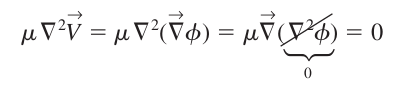
\includegraphics[scale=0.35]{Section_Files/S3-imagenes-Jhon/0060.png}
%\caption{.}
%\end{figure}
%{\tiny Mecánica de fluidos por Yunus A. Cengel, John M. Cimbala, pág. 507}
%\end{frame}

%***************************

%\begin{frame}{Deducción de la ecuación de Bernoulli en regiones irrotacionales de flujo}
%\justifying
%\begin{figure}[H]
%\centering
%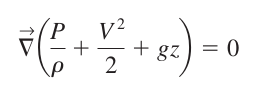
\includegraphics[scale=0.35]{Section_Files/S3-imagenes-Jhon/0062.png}
%\caption{}
%\end{figure}
%{\tiny Mecánica de fluidos por Yunus A. Cengel, John M. Cimbala, pág. 507}
%\end{frame}

%***************************

%\begin{frame}{Regiones irrotacionales bidimensionales de flujo}
%\justifying
%En regiones irrotacionales de flujo...
%\\
%{\tiny Mecánica de fluidos por Yunus A. Cengel, John M. Cimbala, pág. 510}
%\end{frame}

%***************************

%\begin{frame}{Regiones de flujo planar irrotacional}
%\justifying
%\begin{figure}[H]
%\centering
%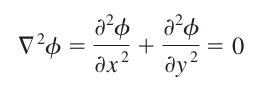
\includegraphics[scale=0.35]{Section_Files/S3-imagenes-Jhon/0072.png}
%\caption{}
%\end{figure}
%{\tiny Mecánica de fluidos por Yunus A. Cengel, John M. Cimbala, pág. 511}
%\end{frame}

%***************************

%\begin{frame}{Regiones irrotacionales de flujo aximétrico}
%\justifying
%\begin{figure}[H]
%\centering
%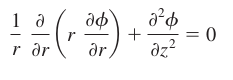
\includegraphics[scale=0.35]{Section_Files/S3-imagenes-Jhon/0081.png}
%\caption{}
%\end{figure}
%{\tiny Mecánica de fluidos por Yunus A. Cengel, John M. Cimbala, pág. 512}
%\end{frame}

%***************************

%\begin{frame}{Resumen de regiones irrotacionales de flujo bidimensional}
%\justifying
%Componentes de velocidad para regiones irrotacionales de flujo bidimensional y estacionario de fluido incompresible en términos de función potencial de velocidad y función de corriente en varios sistemas coordenados.
%\begin{figure}[H]
%\centering
%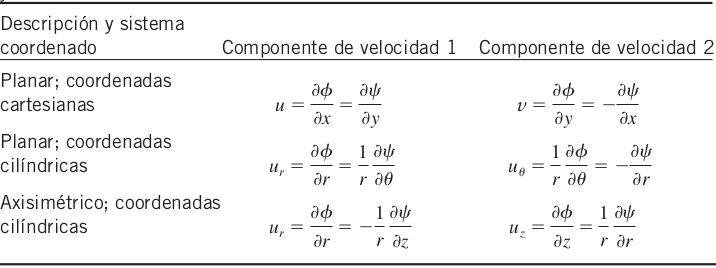
\includegraphics[scale=0.35]{Section_Files/S3-imagenes-Jhon/0088.png}
%\caption{}
%\end{figure}
%{\tiny Mecánica de fluidos por Yunus A. Cengel, John M. Cimbala, pág. 513}
%\end{frame}

%***************************

%\begin{frame}{Superposición de flujo en regiones irrotacionales}
%\justifying
%\begin{figure}[H]
%\centering
%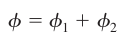
\includegraphics[scale=0.35]{Section_Files/S3-imagenes-Jhon/0091.png}
%\caption{Superposición de dos campos de flujo irrotacional}
%\end{figure}
%{\tiny Mecánica de fluidos por Yunus A. Cengel, John M. Cimbala, pág. 451}
%\end{frame}

%***************************

%\begin{frame}{Flujo planares irrotacionales elementales}
%\justifying
%La superposición permite sumar dos o más soluciones simples de flujo irrotacional, para crear un campo de flujo más complejo (y con la esperanza de ser más significativo físicamente). Por lo tanto, es útil establecer una colección de flujos irrotacionales que sirvan como bloques de la construcción elemental con los que se pueda construir una diversidad de flujos más prácticos...
%\\
%{\tiny Mecánica de fluidos por Yunus A. Cengel, John M. Cimbala, pág. 514}
%\end{frame}


%***************************

%\begin{frame}{Flujo irrotacional formados por superposición}
%\justifying
%Ahora se tiene un conjunto de flujos irrotacionales de bloques de construcción, y se está listo para construir algunos campos de flujo irrotacionales más interesantes mediante la técnica de superposición.
%{\tiny Mecánica de fluidos por Yunus A. Cengel, John M. Cimbala, pág. 521}
%\end{frame}

%***************************

%\begin{frame}{Superposición de un sumidero lineal y un vórtice lineal}
%\justifying
%\begin{figure}[H]
%\centering
%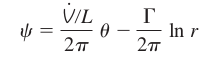
\includegraphics[scale=0.35]{Section_Files/S3-imagenes-Jhon/0132.png}
%\caption{Superposición.}
%\end{figure}
%{\tiny Mecánica de fluidos por Yunus A. Cengel, John M. Cimbala, pág. 521}
%\end{frame}

%***************************

%\begin{frame}{Superposición de un flujo uniforme y un doblete: flujo sobre un cilindro circular}
%\justifying
%\begin{figure}[H]
%\centering
%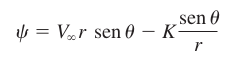
\includegraphics[scale=0.35]{Section_Files/S3-imagenes-Jhon/0137.png}
%\caption{Superposición.}
%\end{figure}
%{\tiny Mecánica de fluidos por Yunus A. Cengel, John M. Cimbala, pág. 522}
%\end{frame}

%***************************

%\begin{frame}{06. La aproximación de capa límite}
%\justifying

%\begin{figure}
%\centering
%\subfloat[Entre la ecuación de Euler (que permite el deslizamiento en las paredes) y la ecuación de Navier-Stokes (que apoya la condición de no deslizamiento) existe un gran vacío.]{
%\label{f:imagen01}
%
\includegraphics[scale=0.20]{Section_Files/S3-imagenes-Jhon/0163.png}}
%\subfloat[La aproximación de capa límite tiende un puente entre ese vacío.]{
%\label{f:imagen02}
%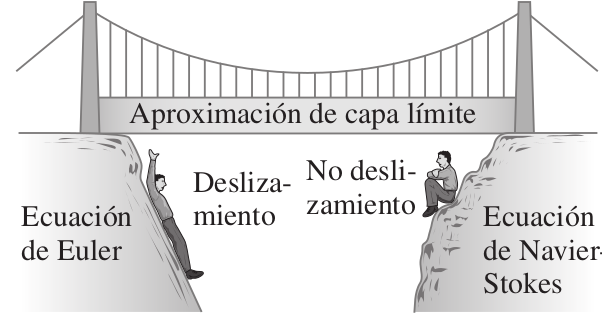
\includegraphics[scale=0.20]{Section_Files/S3-imagenes-Jhon/0164.png}}
%\caption{Imagenes}
%\label{f:imagenes01}

%\end{figure}

%{\tiny Mecánica de fluidos por Yunus A. Cengel, John M. Cimbala, pág. 451}
%\end{frame}

%***************************

%\begin{frame}{Ecuaciones de la capa límite}
%\justifying
%\begin{figure}[H]
%\centering
%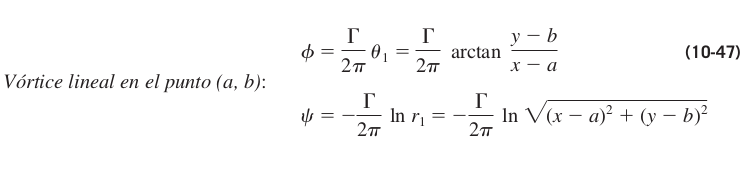
\includegraphics[scale=0.25]{Section_Files/S3-imagenes-Jhon/0123.png}
%\caption{Sistema coordenado para capa límite de flujo sobre un cuerpo; $ x $ sigue la superficie y, por lo general, se establece en cero el punto de estancamiento frontal del cuerpo, y $ y $ localmente es normal a la superficie en todas partes.}
%\end{figure}
%{\tiny Mecánica de fluidos por Yunus A. Cengel, John M. Cimbala, pág. 535}
%\end{frame}

%***************************

%\begin{frame}{El procedimiento de capa límite}
%\justifying
%\begin{figure}[H]
%\centering
%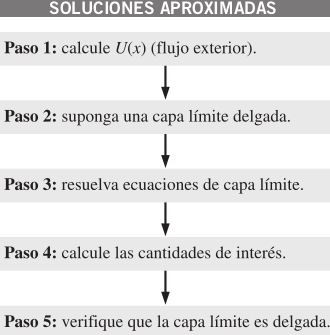
\includegraphics[scale=0.25]{Section_Files/S3-imagenes-Jhon/0202.png}
%\caption{Resumen del procedimiento de capa límite, para capas límite bidimensionales de flujo estacionario e incompresible en el plano $xy$.}
%\end{figure}
%{\tiny Mecánica de fluidos por Yunus A. Cengel, John M. Cimbala, pág. 540}
%\end{frame}

%***************************

%\begin{frame}{Espesor de desplazamiento}
%\justifying
%\begin{figure}[H]
%\centering
%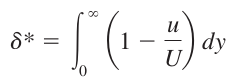
\includegraphics[scale=0.25]{Section_Files/S3-imagenes-Jhon/0211.png}
%\caption{Espesor de desplazamiento}
%\end{figure}
%\\
%{\tiny Mecánica de fluidos por Yunus A. Cengel, John M. Cimbala, pág. 544}
%\end{frame}

%***************************

%\begin{frame}{Espesor de la cantidad de movimiento}
%\justifying
%\begin{figure}[H]
%\centering
%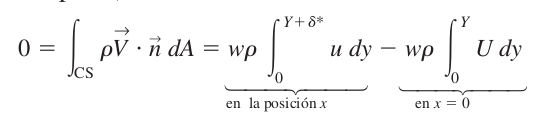
\includegraphics[scale=0.25]{Section_Files/S3-imagenes-Jhon/0219.png}
%\caption{Espesor de desplazamiento}
%\end{figure}
%{\tiny Mecánica de fluidos por Yunus A. Cengel, John M. Cimbala, pág. 547}
%\end{frame}

%***************************

%\begin{frame}{Capa límite turbulenta sobre una placa plana}
%\justifying
%\begin{figure}[H]
%\centering
%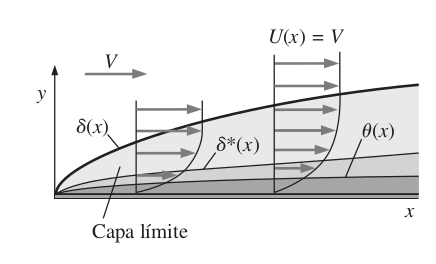
\includegraphics[scale=0.25]{Section_Files/S3-imagenes-Jhon/0231.png}
%\caption{Para una capa límite laminar sobre placa plana, el espesor de desplazamiento es 35.0 por ciento de $ \delta $, y el espesor de la cantidad de movimiento es 13.5 por ciento de $ \delta $. }
%\end{figure}
%{\tiny Mecánica de fluidos por Yunus A. Cengel, John M. Cimbala, pág. 548}
%\end{frame}

%***************************

%\begin{frame}{Capas límite con gradientes de presión}
%\justifying
%\begin{figure}[H]
%\centering
%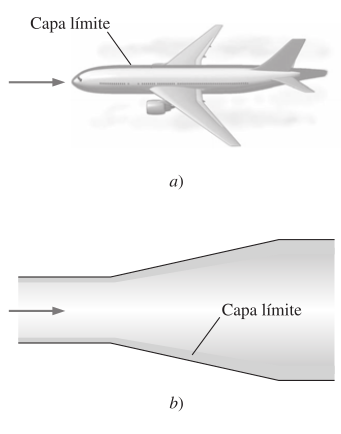
\includegraphics[scale=0.25]{Section_Files/S3-imagenes-Jhon/0245.png}
%\caption{Las capas limite con gradientes de presión distintos de cero ocurren tanto en flujos externos como en internos: a) capa límite que se forma a lo largo del fuselaje de un avión y hacia la estela, y b) capa límite que crece a lo largo de la pared de un difusor (en abmos casos está exagerado el espesor de la capa límite).}
%\end{figure}
%{\tiny Mecánica de fluidos por Yunus A. Cengel, John M. Cimbala, pág. 554}
%\end{frame}

%***************************

%\begin{frame}{Técnica de la integral de la cantidad de movimiento para capas límite}
%\begin{figure}[H]
%\centering
%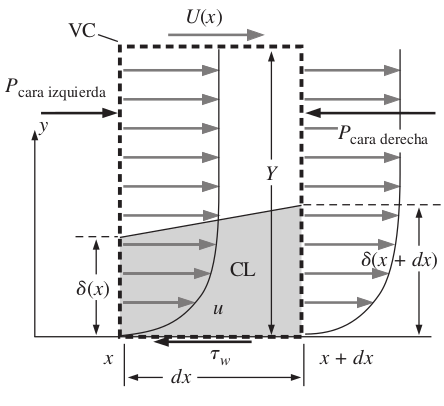
\includegraphics[scale=0.25]{Section_Files/S3-imagenes-Jhon/0259.png}
%\caption{Volumen de control (línea negra punteada gruesa) que se usa en la deducción de la ecuación integral de la cantidad de movimiento (CL se refiere a capa límite.}
%\end{figure}
%{\tiny Mecánica de fluidos por Yunus A. Cengel, John M. Cimbala, pág. 559}
%\end{frame}

%********************


\appendix
\section{Referencias}

\begin{frame}{Referencias}
\begin{thebibliography}{8}

\beamertemplatebookbibitems
\bibitem{Author00}
Web Programming with html5, css, and javascript
\newblock{\em Dean, John}.
\newblock{Jones \& Bartlett Learning (2019)}


\end{thebibliography}
\end{frame}

\begin{frame}{Referencias}
\begin{thebibliography}{8}
\beamertemplatebookbibitems

\bibitem{Author01}
Learn to Code HTML and CSS: Develop and Style Websites
\newblock{\em Howe, Shay}.
\newblock{New Riders, 2014}

\end{thebibliography}
\end{frame}

\end{document}